\chapter{基于聚类的频率分析攻击方法}
\label{sec:ClusteringAttack}

本章放松了基于分布的频率分析攻击中的攻击者的攻击条件要求,提出了基于聚类的频率分析攻击,它不需要使用明文数据块的细粒度排序信息。相反,它利用相似性这一属性来推断来自相似的数据段(即,由数据块块聚合形成的更大的数据单元)的原始数据块,而不依赖于每个数据段中的数据块的排序。 本章首先介绍相似性的概念,然后展示如何使该属性进行推理攻击。

\section{背景知识}
\label{sec:similarity}

\subsection{min-wise independence条件}

对于min-wise independence置换族有如下定义:设$S_n$是$n$元集合$[n]$上所有置换组成的n元对称群。称置换族$F \subseteq S_n$满足min-wise independence条件是指:对任意$X=\{x_1,x_2,\cdots,x_m\}\in[n]$和任意$x_i-inX$,从集合$F$中随机、均匀地选取函数$h$,计算$H(X)=\{h(x_1),h(x_2),\cdots,h(x_m),\}$,有下式成立:
\begin{equation}
    \label{eq:min-wise independence}
    Pr(min(H(X)) = h(x_i) ) = \frac{1}{|X|}
\end{equation}

即$X$中的所有元素在$h$的作用下都有相等的概率成为$H(X)$中的最小元。在实际应用中,完全满足min-wise independence条件的哈希函数很难实现,通常使用近似满足min-wise independence条件的哈希函数即可。

\subsection{Broder定理}
Broder定理\cite{broder1997resemblance}的定义为:两集合$S_1$和$S_2$,$H(S_i)=\{h(x_k)|\forall x_k \in S_i \}$,h是满足min-wise independence条件的哈希函数,$min(S_i)$代表集合$S_i$中的最小元,则

\begin{equation}
    \label{eq:broder}
    \Pr[\min\{{\rm H}(S_1)\} = \min\{{\rm H}(S_2)\} ] = \frac{|S_1 \cap S_2|}{|S_1 \cup S_2|}
\end{equation}

\subsection{相似性}
相似性\cite{bhagwat2009extreme}指出来自同一来源的备份文件可能类似并且共享大部分相同的数据块。 备份文件之间的相似性可以通过Broder定理\cite{broder1997resemblance}来量化。具体来说,如果将每个文件视为一个数据块的集合$S$(即忽略它们的顺序),Broder定理指出如果两组数据块共享相同的最小数据块哈希值的概率很高,则两个集合包含的数据块可能大部分都相同,反之亦然:
 
\begin{eqnarray}
	\Pr[\min\{{\rm H}(S)\} = \min\{{\rm H}(S')\} ] = \frac{|S \cap S'|}{|S \cup S'|}
	\label{eq:similary}
\end{eqnarray}

其中${\rm H}(\cdot)$是一个从min-wise independence置换族中随机统一选择的哈希函数,$\min\{{\rm H}(S)\}$是$S$的最小数据块的哈希。为了便于描述,本文使用MinHash来表示集合中元素的最小哈希值。


针对重复数据删除的各个方面(性能方面\cite{qin2017design,xia2011silo,bhagwat2009extreme},安全方面\cite{li2017information})的已有工作已经利用了相似性这一属性来保持存储效率。具体来说,它们仅针对共享相同最小数据块哈希的文件(即类似的文件)采用MinHash作为一个数据块集合中所有数据块加密使用的密钥进行重复数据删除。根据Broder定理可以推断得到这类文件可能具有大量相同的数据块,因此这种近似精确的重复数据删除只会导致存储效率的轻微降低。与先前的方法不同\cite{qin2017design,xia2011silo,bhagwat2009extreme,li2017information},本文应用相似性来提高频率分析攻击的有效性。
 
\section{基于聚类的频率分析攻击方法定义}
\label{sec:clustering-attack-description}

现在提出基于聚类的频率分析攻击方法(图:\ref{fig:基于聚类的攻击方法的工作流程}),它基于相似性在加密重复数据删除中推断密文数据块的原始明文数据块。

\begin{figure}[!htb]
    \small
    \centering
    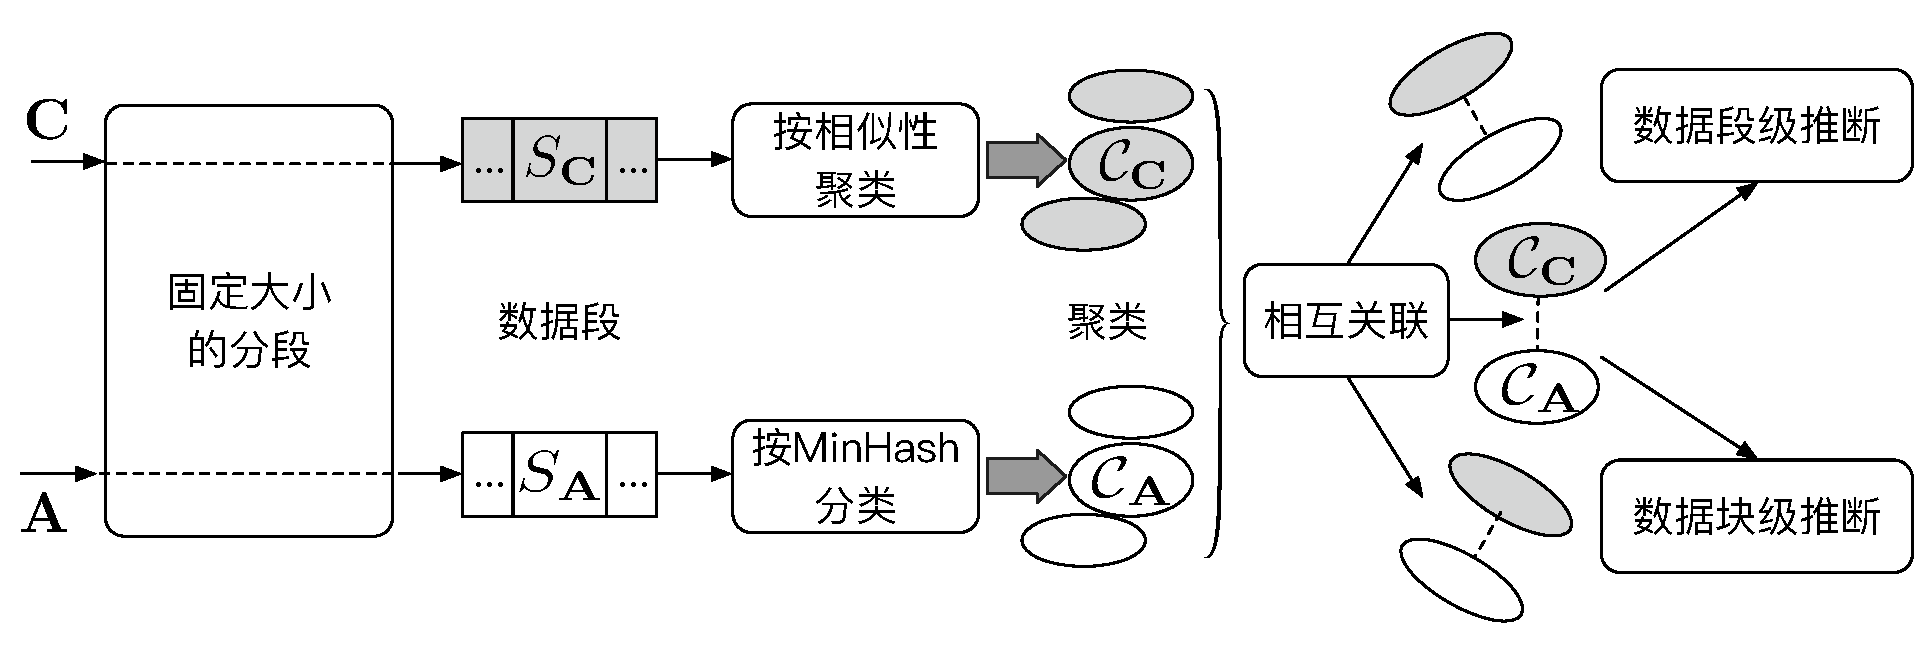
\includegraphics[width=14cm]{ClusteringAttack.eps}
    \caption{基于聚类的攻击方法的工作流程:用MinHash表示明文数据段的最小块散列} 
    \label{fig:基于聚类的攻击方法的工作流程}
\end{figure}

为了利用相似性,我们首先在块流上引入{\ em segmentation}。具体来说,我们将$ \ mathbf {C} $分区为一组粗粒度数据单元,称为{\ em密文段}。每个密文段,由$ S_ \ mathbf {C} $表示,包含$ \ mathbf {C} $中的多个相邻密文。在这项工作中,我们实现了{\ em fixed-size}分段方案,以确保所有密文段具有相同的大小(例如,默认为4MB)。为了兼容性,相同的固定大小分段方案也适用于辅助信息$ \ mathbf {A} $,以便生成多个{\ em明文段},每个段由$ S_ \ mathbf {A} $表示。注意,一些可变大小的分段方案\ cite {lillibridge09,qin17}在其内容与特定模式匹配的块之后识别分段边界,从而解决固定大小分段方案所面临的边界移位问题。但是,我们不能在攻击中使用这些可变大小的分段方案\ cite {lillibridge09,qin17}。原因是密文段中的块的原始内容受到对称加密的保护,我们无法确保密文和明文段的边界匹配相同的模式。这会导致密文和明文段之间不兼容,并且会降低基于群集的攻击所推断的段级数据量(请参阅本节后半部分)。

To exploit similarity, we first introduce {\em segmentation} on a stream of chunks. Specifically, we partition $\mathbf{C}$ into a set of coarse-grained data units, called {\em ciphertext segments}. Each ciphertext segment, denoted by $S_\mathbf{C}$, comprises multiple adjacent ciphertexts in $\mathbf{C}$. In this work, we implement the {\em fixed-size} segmentation scheme to ensure that all ciphertext segments are of the same size (e.g., 4MB by default). For compatibility, the same fixed-size segmentation scheme also applies to the auxiliary information $\mathbf{A}$, so as to generate multiple {\em plaintext segments}, each of which is denoted by $S_\mathbf{A}$. Note that some variable-size segmentation schemes \cite{lillibridge09, qin17}  identify segment boundaries after the chunks whose contents match a specific pattern and thus address the boundary shift problem faced by the fixed-size segmentation scheme. However, we cannot use these variable-size segmentation schemes \cite{lillibridge09, qin17} in the attack. The reason is that the original contents of chunks in ciphertext segments are protected by symmetric encryption, and we cannot ensure that the boundaries for both ciphertext and plaintext segments match the same pattern. This leads to an incompatibility between ciphertext and plaintext segments, and degrades the amount of segment-level data inferred by the clustering-based attack (see the late part of this section).    

We propose to infer ciphertext-plaintext pairs through similar segments. Let $S_\mathbf{M}$ be the original plaintext segment of a ciphertext segment $S_\mathbf{C}$ (i.e., each plaintext in $S_\mathbf{M}$ corresponds to some ciphertext in $S_\mathbf{C}$ and vice versa). According to Broder's theorem, if $S_\mathbf{M}$ shares the same minimum chunk hash, say $h$, with some plaintext segment $S_\mathbf{A}$, then $S_\mathbf{M}$  and $S_\mathbf{A}$ tend to have a large fraction of identical plaintexts. This implies that the ciphertexts in $S_\mathbf{C}$ are likely to be mapped from the plaintexts in  $S_\mathbf{A}$. In other words, we first classify all plaintext segments of $\mathbf{A}$ by their minimum chunk hashes, and obtain multiple {\em plaintext clusters}. Each plaintext cluster, denoted by $\mathcal{C}_\mathbf{A} = \{ S_\mathbf{A} \}$, corresponds to a unique minimum chunk hash shared by its included segments. We also group the ciphertext segments, whose original plaintext segments have the same minimum chunk hash $h$ (i.e., similar), into an identical {\em ciphertext cluster}, denoted by $\mathcal{C}_\mathbf{C} = \{ S_\mathbf{C} \}$. Then, we infer the original data of $\mathcal{C}_\mathbf{C}$ from some $\mathcal{C}_\mathbf{A}$ that corresponds to  $h$.    

We propose a {\em clustering} scheme to group similar ciphertext segments. A na\"{i}ve approach is to classify segments by their minimum chunk hashes, but it does not work on ciphertext segments, whose original contents are protected by symmetric encryption. We address the classification issue based on Broder's theorem.   
  
Our insight is that if two ciphertext segments have a large fraction of identical ciphertexts, then  they correspond to the same minimum chunk hash with a high probability. The reason is that deterministic encryption preserves the cardinalities of union and intersection of plaintext segments, based on which we can use Broder's theorem to learn the equivalence of their minimum chunk hashes.    

In this work, we define the {\em clustering distance} $d(S_\mathbf{C}, S_\mathbf{C}')$ of any two ciphertext segments $S_\mathbf{C}$ and $S_\mathbf{C}'$ by one minus the fraction of their identical ciphertexts:

\begin{eqnarray}
d(S_\mathbf{C}, S_\mathbf{C}') = 1 - \frac{|S_\mathbf{C} \cap S_\mathbf{C}'|}{|S_\mathbf{C} \cup S_\mathbf{C}'|}. \nonumber
\end{eqnarray}

Note that identical ciphertexts may repeat in $S_\mathbf{C}$ or $S_\mathbf{C}'$, and $|S_\mathbf{C} \cap S_\mathbf{C}'|$ and $|S_\mathbf{C} \cup S_\mathbf{C}'|$ return the number of {\em unique} ciphertexts in their  intersection and union, respectively. Clearly,  the smaller $d(S_\mathbf{C}, S_\mathbf{C}')$ is, the more likely are $S_\mathbf{C}$ and $S_\mathbf{C}'$ to correspond to the same minimum chunk hash. Then, we adopt the {\em agglomerative hierarchical clustering (AHC)} \cite{johnson67} to aggregate similar ciphertext segments based on their distance information.  Specifically, we start with eash ciphertext segment in its own singleton cluster, and iteratively combine the two closest clusters based on the maximum distance of their ciphertext segments. We configure a parameter $k$, and stop the iterated combination when the maximum distance of ciphertext segments in the two cloestclusters is greater than $k$.  

For each aggregated ciphertext cluster $\mathcal{C}_\mathbf{C}$, we relate it to some plaintext cluster $\mathcal{C}_\mathbf{A}$ with frequency analysis, while taking frequency distribution into account. This is based on the observation that identical ciphertexts (resp. plaintexts) may  repeat in the same or different ciphertext (resp. plaintext) segments and identical ciphertext (resp. plaintext) segments may also repeat in the same ciphertext (resp. plaintext) cluster. We propose to examine the frequency distribution of the logical ciphertexts or plaintexts in each cluster, and perceive that the frequency distributions for similar clusters (i.e., correspond to the same minimum chunk hash) are also likely to be similar. 
 
We proceed the frequency analysis scheme as follows. First, we  sort available ciphertext and plaintext clusters by the total number of logical  ciphertexts and plaintexts they include, respectively. Then, we count an associative array $\mathbf{F}$ that stores the frequency of each unique ciphertext or plaintext in  corresponding cluster. Based on $\mathbf{F}$, we compute the probability that a  ciphertext $C$ exists in a ciphertext cluster $\mathcal{C}_\mathbf{C}$ and further the entropy of $\mathcal{C}_\mathbf{C}$:        

\begin{eqnarray*}
    \Pr[C \in \mathcal{C}_\mathbf{C}] = \frac{\mathbf{F}[\mathcal{C}_\mathbf{C}][C]}{\sum_{C' \in \mathcal{C}_\mathbf{C}} \mathbf{F}[\mathcal{C}_\mathbf{C}][C']}, \\
    e(\mathcal{C}_\mathbf{C}) = \sum_{C \in \mathcal{C}_\mathbf{C}} \log_2 \frac{1}{\Pr[C \in \mathcal{C}_\mathbf{C}]},  
    % e(\mathcal{C}_\mathbf{M}) = \sum_{M \in \mathbf{F}[\mathcal{C}_\mathbf{M}]} \log_2 \frac{\mathbf{F}[\mathcal{C}_\mathbf{M}][M]}{a} 
\end{eqnarray*}

where $\mathbf{F}[\mathcal{C}_\mathbf{C}][C]$  stores the frequency of $C$ in $\mathcal{C}_\mathbf{C}$. Similarly, we  compute the entropy $e(\mathcal{C}_\mathbf{A})$ for the plaintext cluster $\mathcal{C}_\mathbf{A}$. Like the distribution-based attack (see Section~\ref{sec:distribution-attack-description}), we configure the frequency analysis scheme with the parameters $(u, r, t)$, and infer that the ciphertext cluster $\mathcal{C}_\mathbf{C}$ is similar to a plaintext cluster $\mathcal{C}_\mathbf{A}$, if they satisfy the following requirements:
  
\begin{itemize}[leftmargin=*]
    \item  The rank of $\mathcal{C}_\mathbf{C}$ is not larger than $u$.
    \item  The rank difference of $\mathcal{C}_\mathbf{C}$ and $\mathcal{C}_\mathbf{A}$ is not larger than $r$.  
    \item  The difference of $e(\mathcal{C}_\mathbf{C})$ and $e(\mathcal{C}_\mathbf{A})$ is the smallest and also not larger than $t$.
\end{itemize}

Then, for each pair $(\mathcal{C}_\mathbf{C}, \mathcal{C}_\mathbf{A})$ of similar clusters, we infer ciphertext-plaintext pairs in two levels. 
\begin{itemize}[leftmargin=*]
    \item {\bf Segment-level inference:}
        If $\mathcal{C}_\mathbf{C}$ and $\mathcal{C}_\mathbf{A}$ have the same number of logical chunks (i.e., ciphertexts or plaintexts), as well as an identical entropy, this implies that $\mathcal{C}_\mathbf{C}$ is exactly mapped from $\mathcal{C}_\mathbf{A}$ with a high probability. In this case, we operate attack on the coarse-grained {\em segment} level. Specifically, we first compute the entropies of each ciphertext segment $S_\mathbf{C}$ in $\mathcal{C}_\mathbf{C}$ and each plaintext segment $S_\mathbf{A}$ in $\mathcal{C}_\mathbf{A}$, based on the frequency distributions of their ciphertexts and plaintexts, respectively. 
         We infer that $S_\mathbf{C}$ is mapped from  $S_\mathbf{A}$, if the total numbers of logical chunks, as well as the entropies, of $S_\mathbf{C}$ and $S_\mathbf{A}$ are identical. Our evaluation shows that the segment-level inference contributes most of the correctly inferred contents in the
        clustering-based attack (see
        Section~\ref{sec:experiment-clustering}). It is also possible to further recover each plaintext in these inferred segments with additional adversarial knowledge (e.g., ordering). 
    \item {\bf Chunk-level inference:}
        If $\mathcal{C}_\mathbf{C}$ and $\mathcal{C}_\mathbf{A}$ have different numbers of logical chunks or entropies, we apply frequency analysis to operate attack on the fine-grained {\em chunk} level. Specifically, we sort all unique ciphertexts and plaintexts by their frequencies in $\mathcal{C}_\mathbf{C}$ and $\mathcal{C}_\mathbf{A}$, respectively, and infer ciphertext-plaintext pairs based on frequency ranks.  
        However, we find the chunk-level inference does not perform well in our experimental dataset. The possible reason is each cluster includes a large number of logical chunks, which degrades the effectiveness of  frequency analysis. Even so, we expect the chunk-level inference can recover more ciphertext-plaintext pairs in practice, especially when the number of logical chunks in some clusters is limited.   
\end{itemize}

\subsection{本章小结}

To summarize, the clustering-based attack exploits similarity, and launches frequency analysis in similar clusters to infer ciphertext-plaintext pairs. In addition to  $u$, $r$ and $t$, it is configured by the parameter $k$, which specifies the upper bound distance in combining the closest clusters.   

Although possibly affected by the boundary shift of fixed-size segments, we argue that the clustering-based attack is severe against VM disk images. Specifically, a flat VM image file is allocated of a fixed size at the time it is created, and such size cannot be changed during its lifetime. All unused regions in a VM image are initially filled with  zero chunks, which can be further re-written for storing additional data in the image. In Section \ref{sec:experiment-clustering}, we examine the effectiveness of the clustering-based attack against VM images.


